\newpage
\subsection{Utilizzo dell'applicativo}
Alla fine della fase di codifica, assistito dal tutor, ho creato gli eseguibili (installers oppure pacchetti, a seconda della piattaforma), attraverso Electron Forge.\\
Allo stato da me raggiunto, ENGaming può essere utilizzato con:
\begin{itemize}
    \item un PC con installato il driver \gls{displaylink} e uno dei seguenti sistemi operativi: \begin{itemize}
    \item Windows 11 (non necessario installare il driver citato in precedenza, in quanto già presente).
    \item MacOS Ventura.
    \end{itemize}
    \item un ENSign11 da collegare a suddetto PC.
\end{itemize}
Purtroppo non ho potuto testare l'applicativo in altre versioni di Windows o MacOS, a causa della mancanza di tempo nel farlo. Non sono invece stati testati altri device di firma poichè non sono stati considerati come device target, a differenza dell'ENSign11.\\
Su sistemi operativi con kernel Linux, l'applicativo veniva eseguito ma non riconosceva il tablet, costringendo un utilizzo tramite tastiera e mouse e in generale con errori dovuti proprio al non riconoscimento del device.
\newpage
\subsection{Panoramica del prodotto}
Per concludere questa sezione, voglio mostrare il frutto della fase di codifica, partendo dalla schermata iniziale e concludendo con la gestione dell'inattività.\\
La schermata iniziale dell'applicazione comprende:
\begin{itemize}
    \item Il nome dell'applicazione stessa.
    \item L'elenco dei giochi disponibili, sotto forma di icone.
    \item Un'icona per visualizzare i record effettuati.
    \item Un'icona per uscire dall'applicazione.
\end{itemize}
\begin{figure}[h]
    \centering
    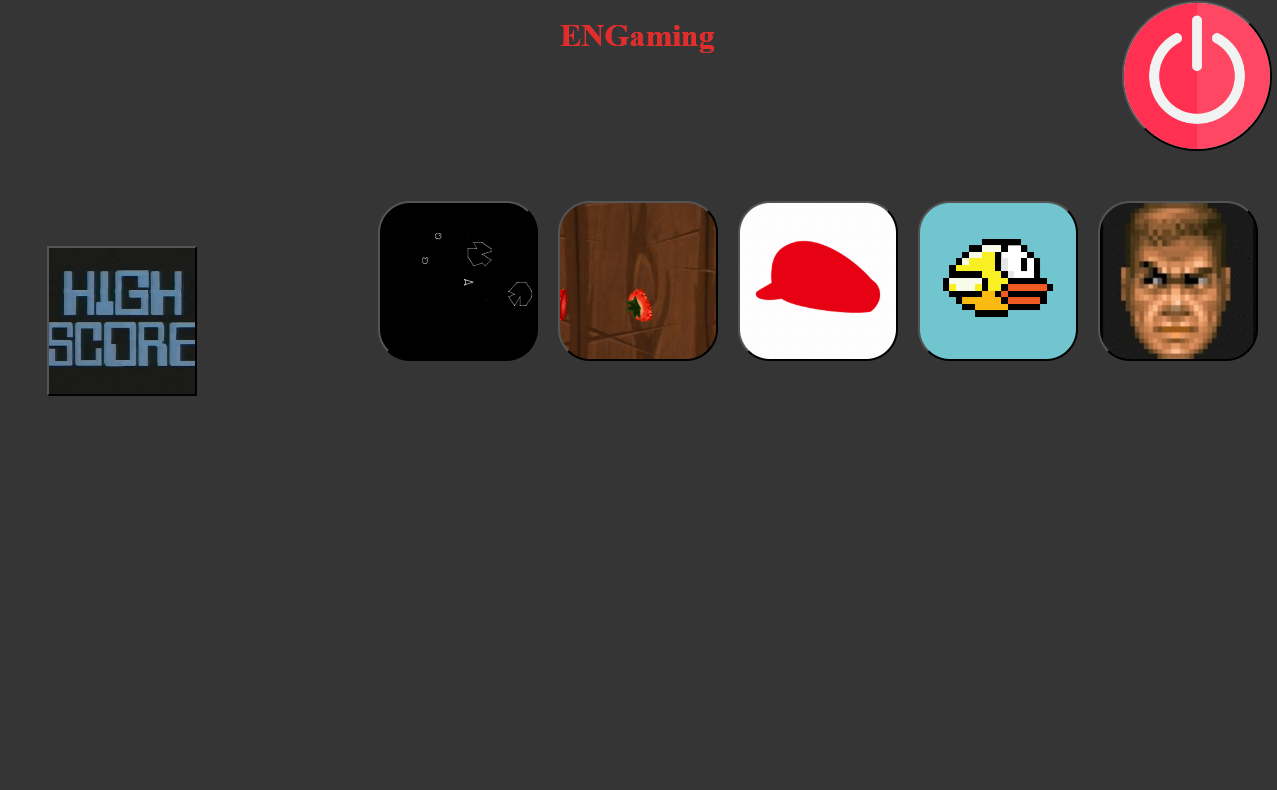
\includegraphics[width=250pt]{images/product/schermataIniziale.png}
    \caption{Schermata iniziale di ENGaming}
    \label{fig:schermataIniziale}
\end{figure}
Ho scelto una visualizzazione il più possibile vicina alle icone per portare un senso di famigliarità, in quanto ENGaming viene usato attraverso uno schermo touch.
\newpage
Atraverso l'icona "High Score", è possibile passare alla visualizzazione dei record.\\
La pagina apposita mostra la lista dei record globale, ovvero mostra tutti i record effettuati senza distinzione di gioco.\\
In particolare, ogni record mostra:
\begin{itemize}
    \item l'utente che ha effettuato il record
    \item il punteggio totalizzato
    \item la data in cui è stato effettuato il record
    \item il gioco in cui è stato effettuato il record
\end{itemize}
\begin{figure}[h]
    \centering
    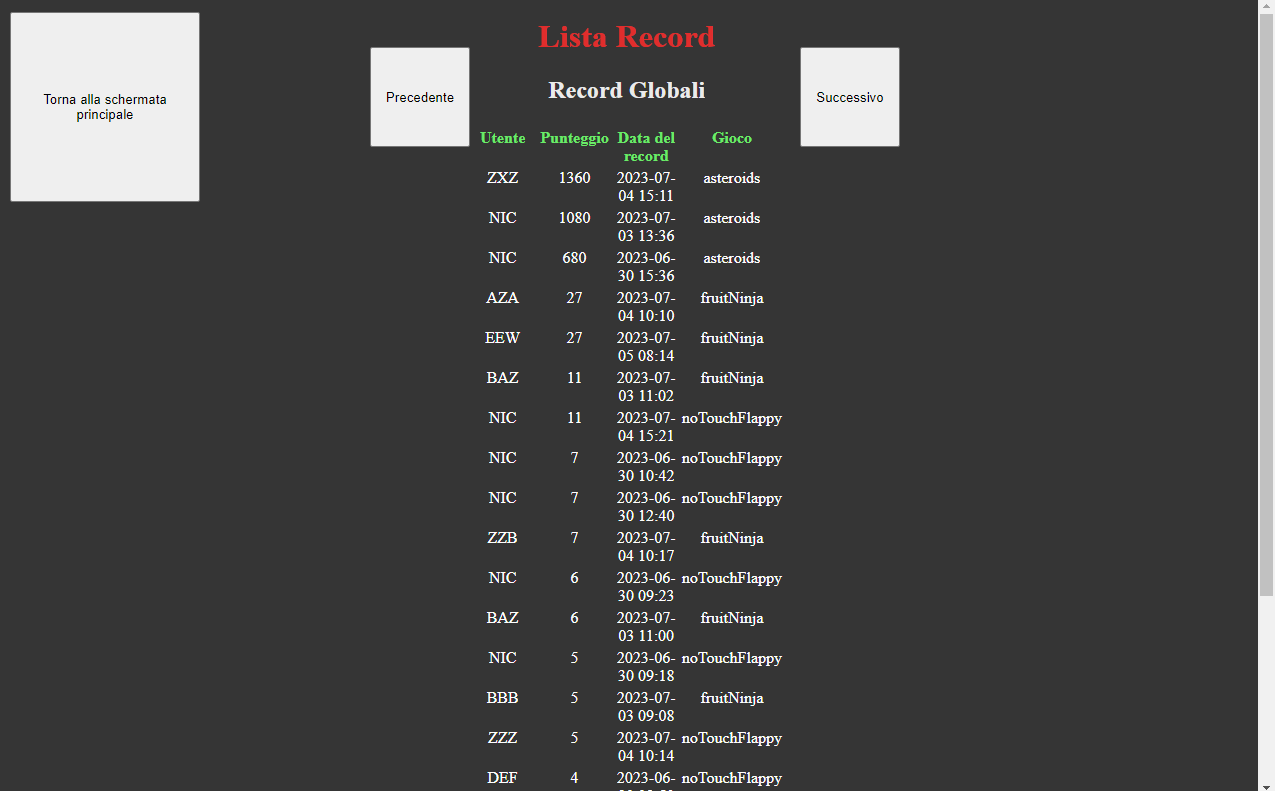
\includegraphics[width=250pt]{images/product/schermataRecord.png}
    \caption{Lista dei record globali}
    \label{fig:schermataRecord}
\end{figure}
Utilizzando i pulsanti "attorno" alla lista, si può passare alla lista dei record per i giochi specifici.\\
Tali liste sono tante quanti i giochi in cui sia stato fatto almeno un record.
La prima e l'ultima lista di questo genere, alla pressione degli appositi pulsante, riportano alla lista globale.
\begin{figure}[h]
    \centering
    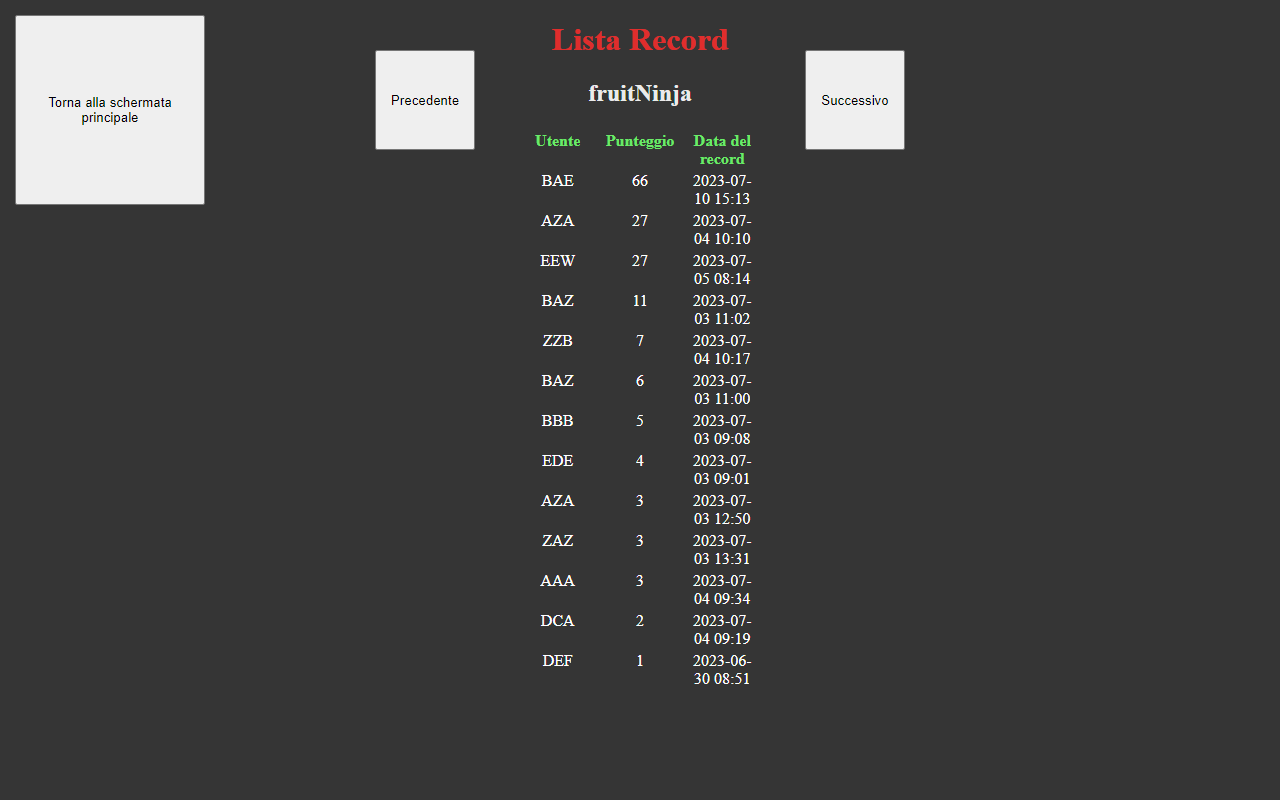
\includegraphics[width=250pt]{images/product/schermataRecordSingoloGioco.png}
    \caption{Esempio di lista per un singolo gioco}
    \label{fig:schermataRecordSingoloGioco}
\end{figure}
\newpage
Ritornando alla schermata iniziale, si può selezionare un gioco attraverso la propria icona.\\
Tale operazione porta alla pagina del gioco stesso, che contiene le informazioni sul gioco stesso, ovvero:
\begin{itemize}
    \item il nome del gioco.
    \item il genere del gioco.
    \item il tipo di input, ovvero se viene utilizzato il controller o il touch/digitalizer.
    \item la descrizione del gioco.
    \item L'elenco degli input, o delle gesture, che il gioco ha.
\end{itemize}
\begin{figure}[h]
    \centering
    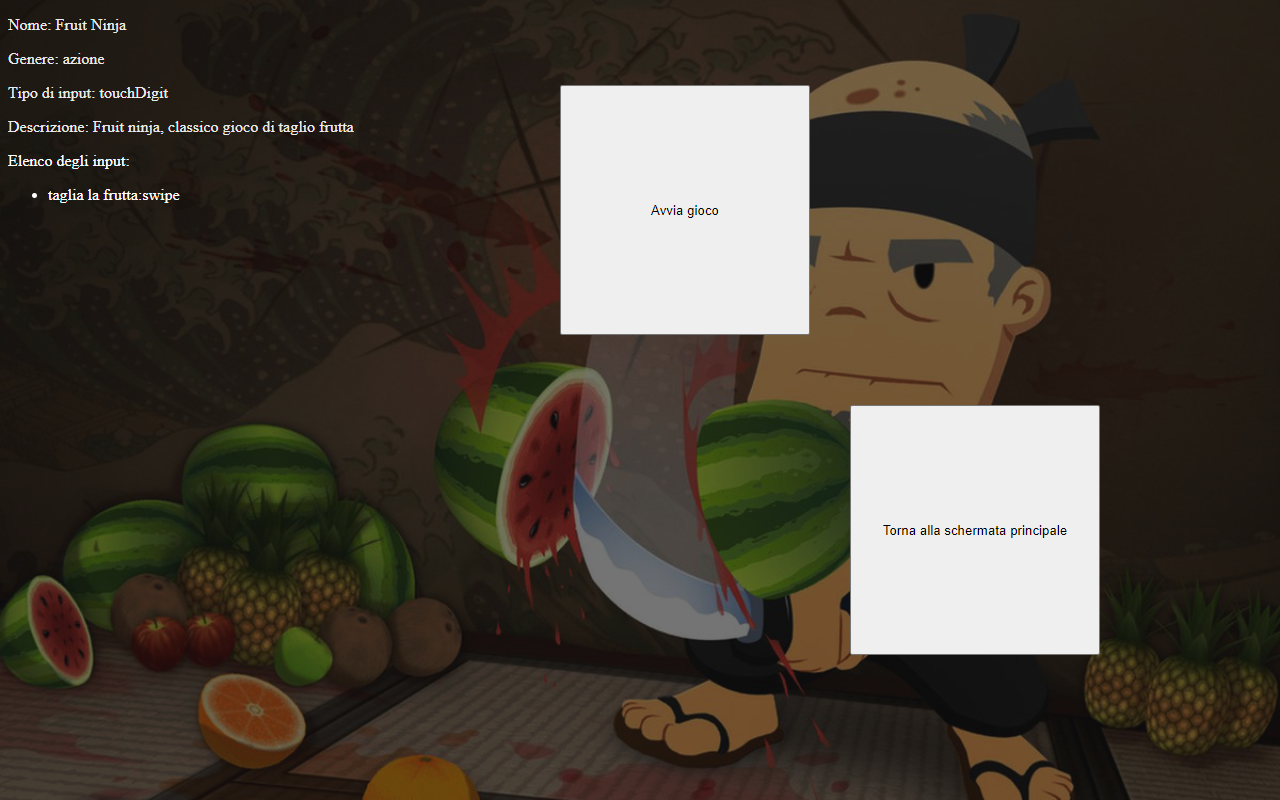
\includegraphics[width=250pt]{images/product/schermataPaginaGioco.png}
    \caption{Esempio di pagina di un gioco}
    \label{fig:schermataPaginaGioco}
\end{figure}
Ovviamente, da questa pagina si può decidere se avviare il gioco o tornare alla schermata principale.\\\\
All'avvio del gioco, si passa attraverso una pagina di caricamento. La pagina in questione è spoglia, in quanto informa semplicemente l'utente dello stato di caricamento.\\
Questa pagina viene visualizzata per 4 secondi, per poi passare all'interfaccia di gioco.
\begin{figure}[h]
    \centering
    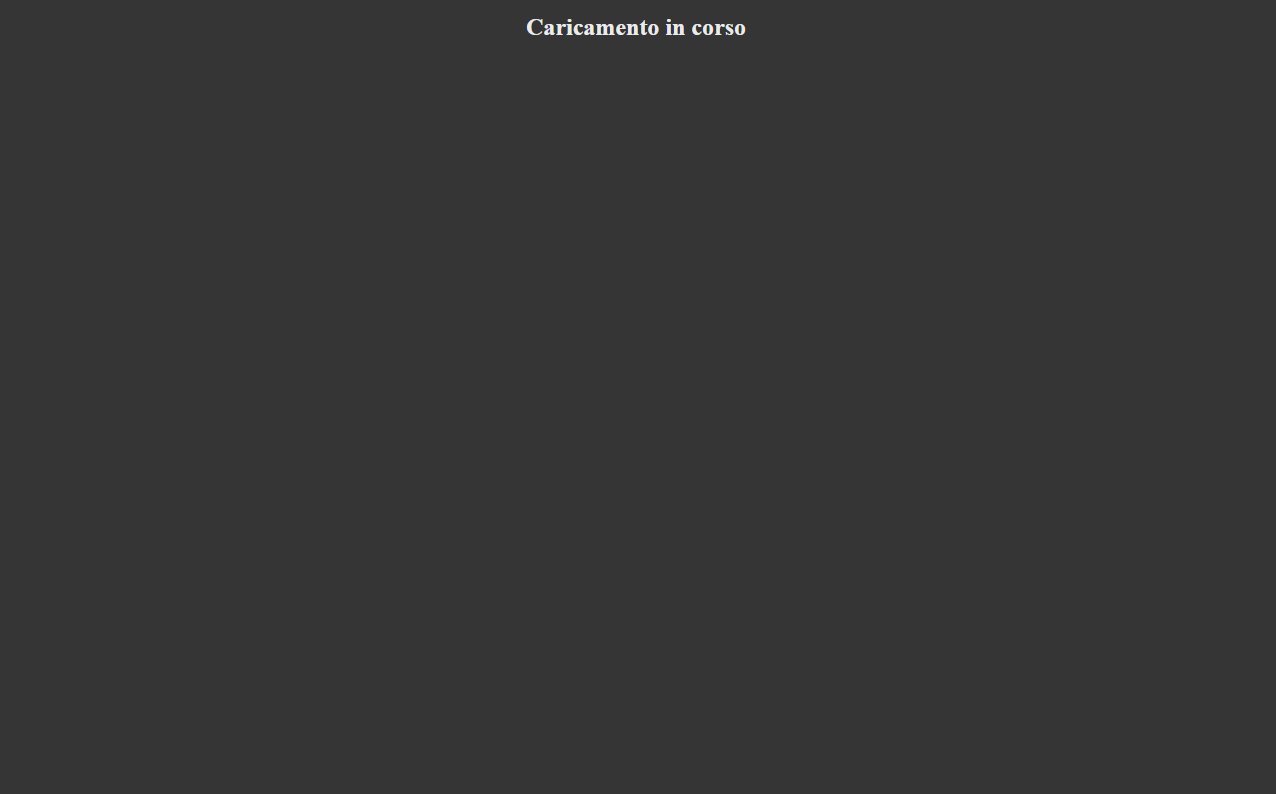
\includegraphics[width=250pt]{images/product/schermataCaricamento.png}
    \caption{Schermata di caricamento}
    \label{fig:schermataCaricamento}
\end{figure}
\newpage
La differenza tra le due tipologie di gioco entra adesso.\\
Infatti, se il gioco prevede l'utilizzo del controller, oltre al gioco stesso si visualizza anche il controller, che dalla struttura di default (spiegata in ControllerMettimiIlLinkOraNonHoCazzi), viene configurato attraverso gli input che il gioco richiede.
\begin{figure}[h]
    \centering
    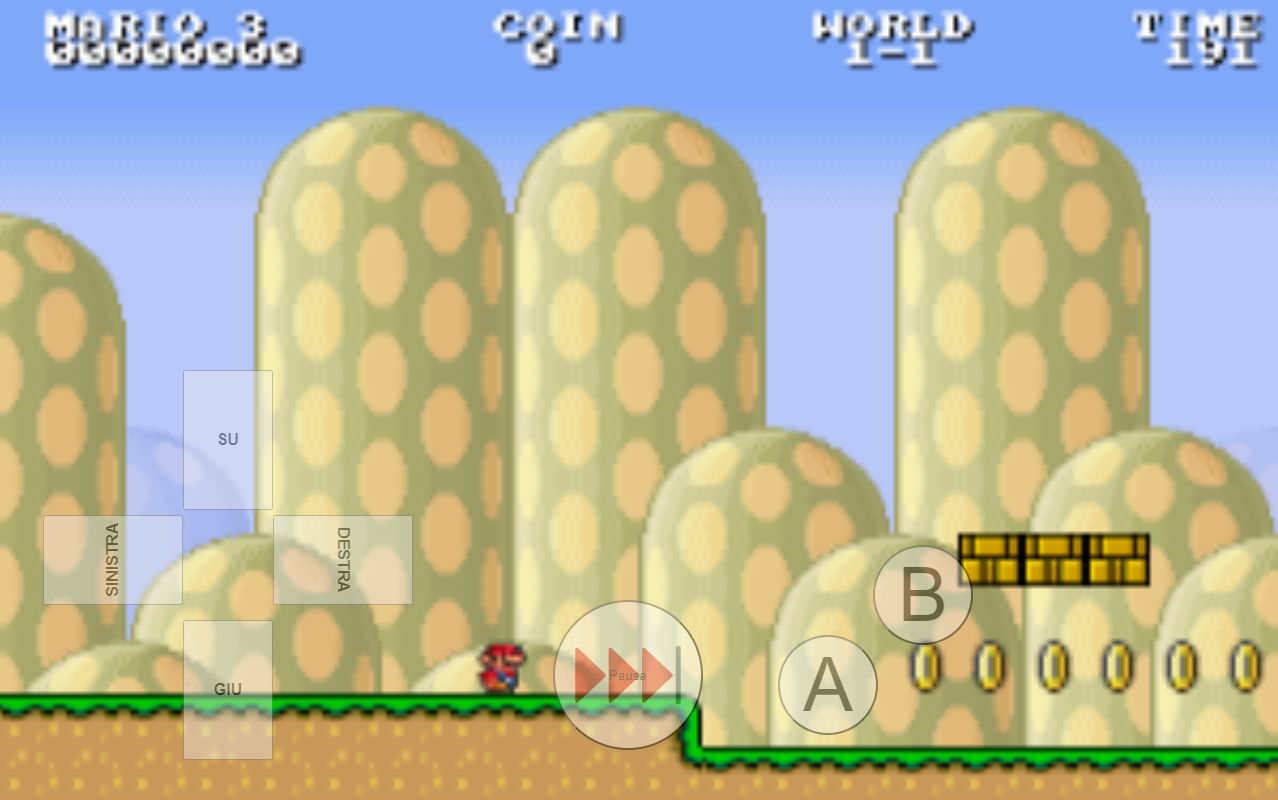
\includegraphics[width=250pt]{images/product/schermataGiocoController.png}
    \caption{Esempio di schermata per un gioco con il controller}
    \label{fig:schermataGiocoController}
\end{figure}
\newpage
\subsubsection{Schermata di gioco-touch/digitalizer}
Nel caso di un gioco che richieda l'uso del touch o del digitalizer, si viene reindirizzati a questa schermata.\\
La schermata è composta dal gioco stesso e dal solo pulsante di pausa, dato che i comandi vengono dati tramite gestures.\\
Il pulsante di pausa è posizionato in modo da intralciare il meno possibile l'utente durante il gioco, al fine di non intaccare l'esperienza d'uso.
\begin{figure}[h]
    \centering
    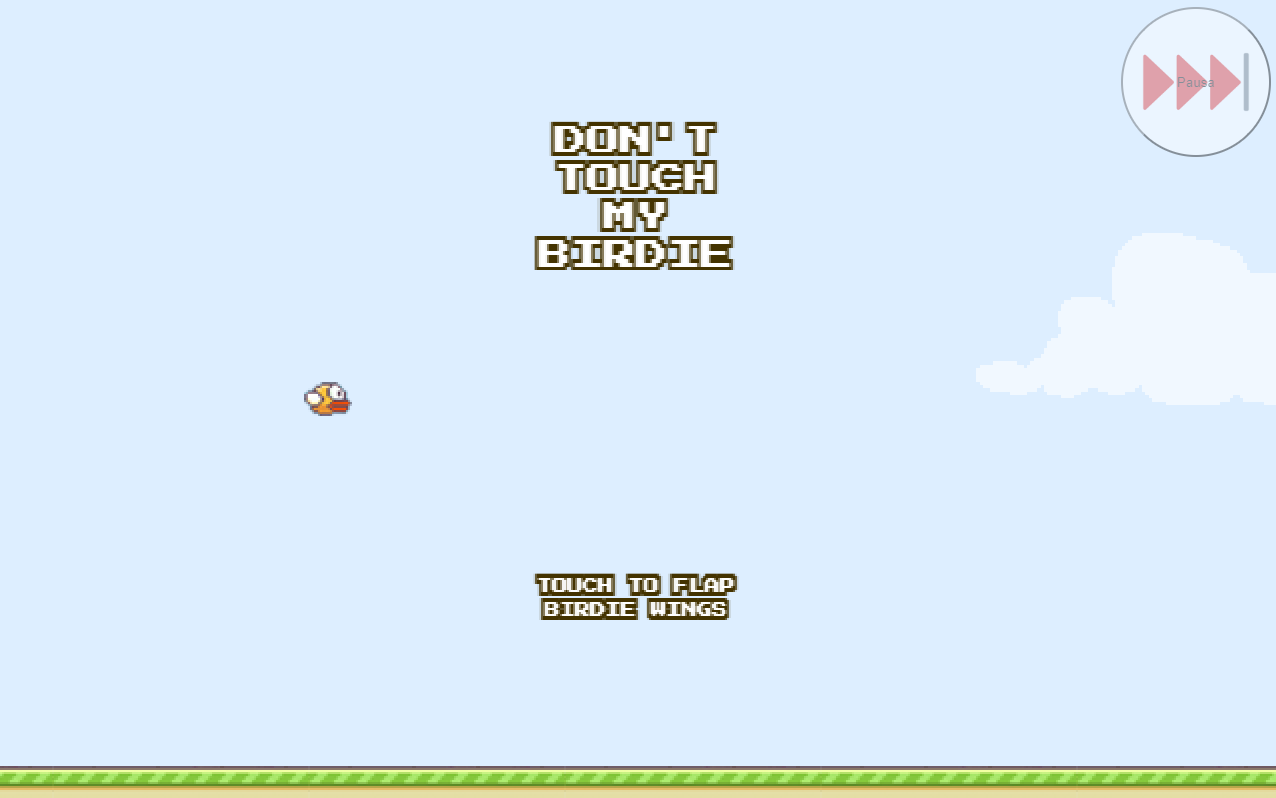
\includegraphics[width=250pt]{images/product/schermataGiocoTouchDigit.png}
    \caption{Esempio di schermata per un gioco con il touch/digitalizer}
    \label{fig:schermataGiocoTouchDigit}
\end{figure}
\newpage
\subsubsection{Pagina di pausa}
Premendo sul pulsante di pausa, si arriva alla schermata apposita.\\
La schermata di pausa, oltre ad informare l'utente dello stato di pausa dell'applicazione, permette di ritornare al gioco attualmente in esecuzione oppure di uscire dal gioco, tornando al menù principale.
\begin{figure}[h]
    \centering
    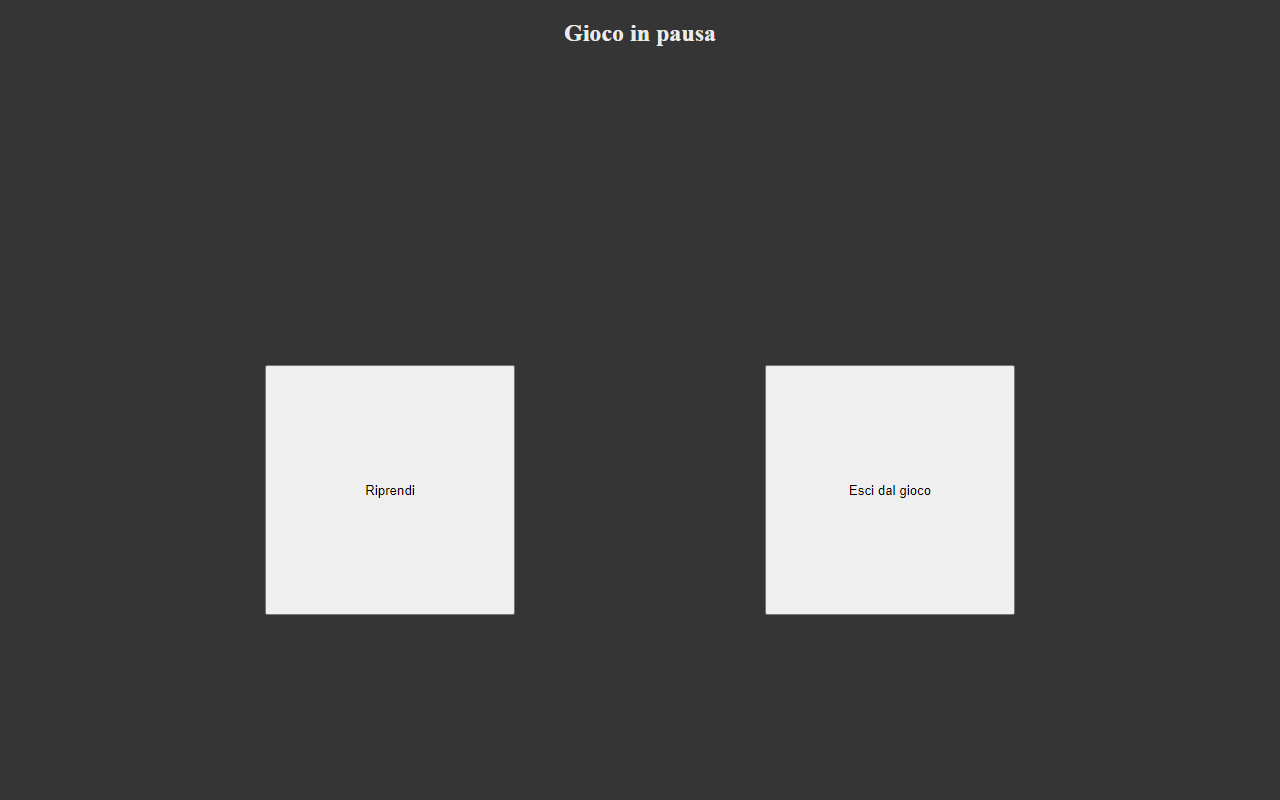
\includegraphics[width=250pt]{images/product/schermataPausaGioco.png}
    \caption{Schermata di pausa}
    \label{fig:schermataPausaGioco}
\end{figure}
\subsubsection{Inattività nei giochi o nella schermata di pausa}
Per quanto accade durante un'eventuale inattività, si rimanda alla sezione di \hyperref[sec:inactivity]{Gestione dell'inattività}
\newpage
\subsection{Realizzazione di un nuovo record}
Se l'utente, durante la sua sessione di gioco (ovvero da quando ha avviato il gioco fino a quando lo ha chiuso) ha effettuato un nuovo record, viene mostrata la schermata di notifica di un nuovo record.
\subsubsection{Pagina di notifica di un nuovo record}
Questa schermata notifica l'utente del compimento di un nuovo record. Il nuovo record è legato al gioco appena concluso.\\
Inoltre, viene chiesto all'utente se desidera salvare il record appena effettuato o se non desidera salvarlo, fornendo i pulsanti per la selezione.
\begin{figure}[h]
    \centering
    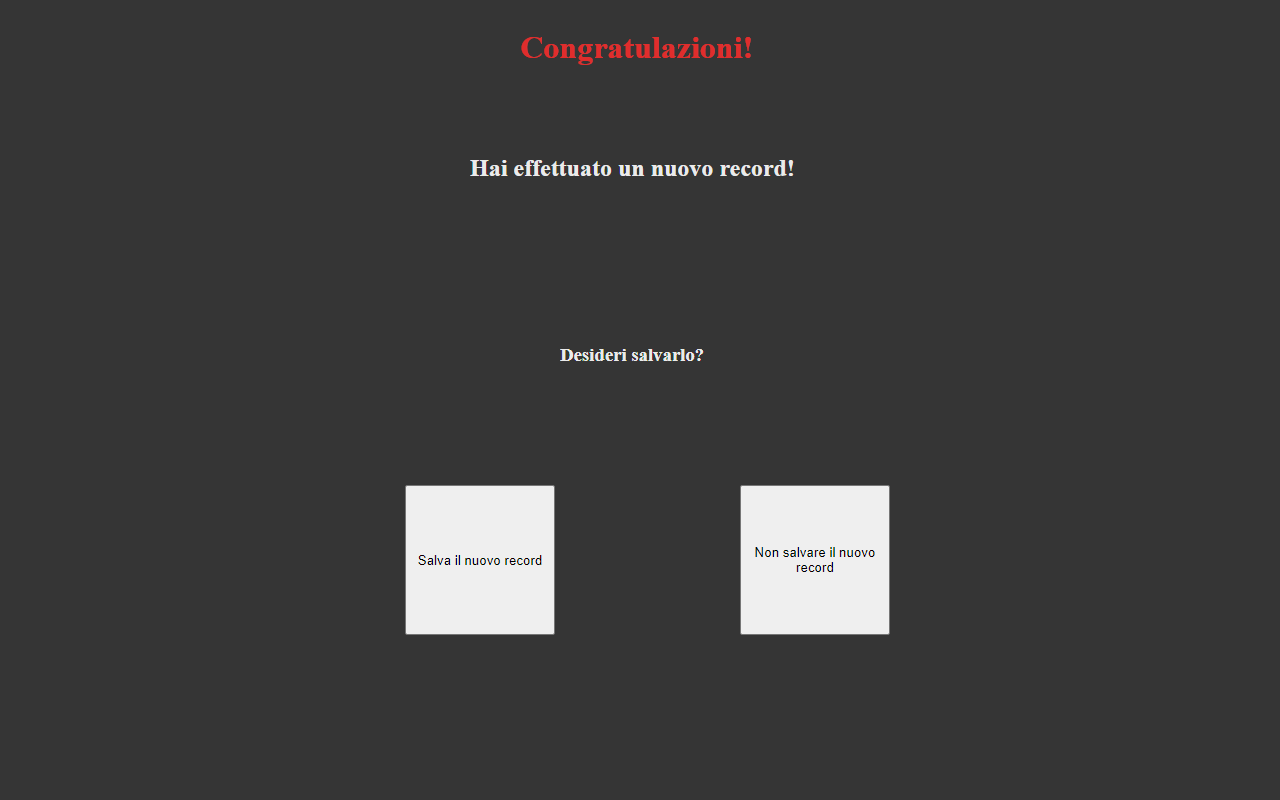
\includegraphics[width=250pt]{images/product/schermataNuovoRecord.png}
    \caption{Schermata di avviso per un nuovo record}
    \label{fig:schermataNuovoRecord}
\end{figure}
\subsubsection{Pagina di inserimento nome-stile arcade}
Nel caso l'utente decidesse di salvare il record, ne viene richiesto l'inserimento del nome attraverso questa schermata.\\
Il nome viene inserito come nei vecchi cabinati arcade, ovvero selezionando tre caratteri da una lista di caratteri. Per la selezione, vengono utilizzati gli appositi pulsanti, situati sopra e sotto ogni singola lettera.\\
Alla conferma, il nome viene messo sul record e salvato, e sarà dunque visibile nell'apposita schermata.
\begin{figure}[h]
    \centering
    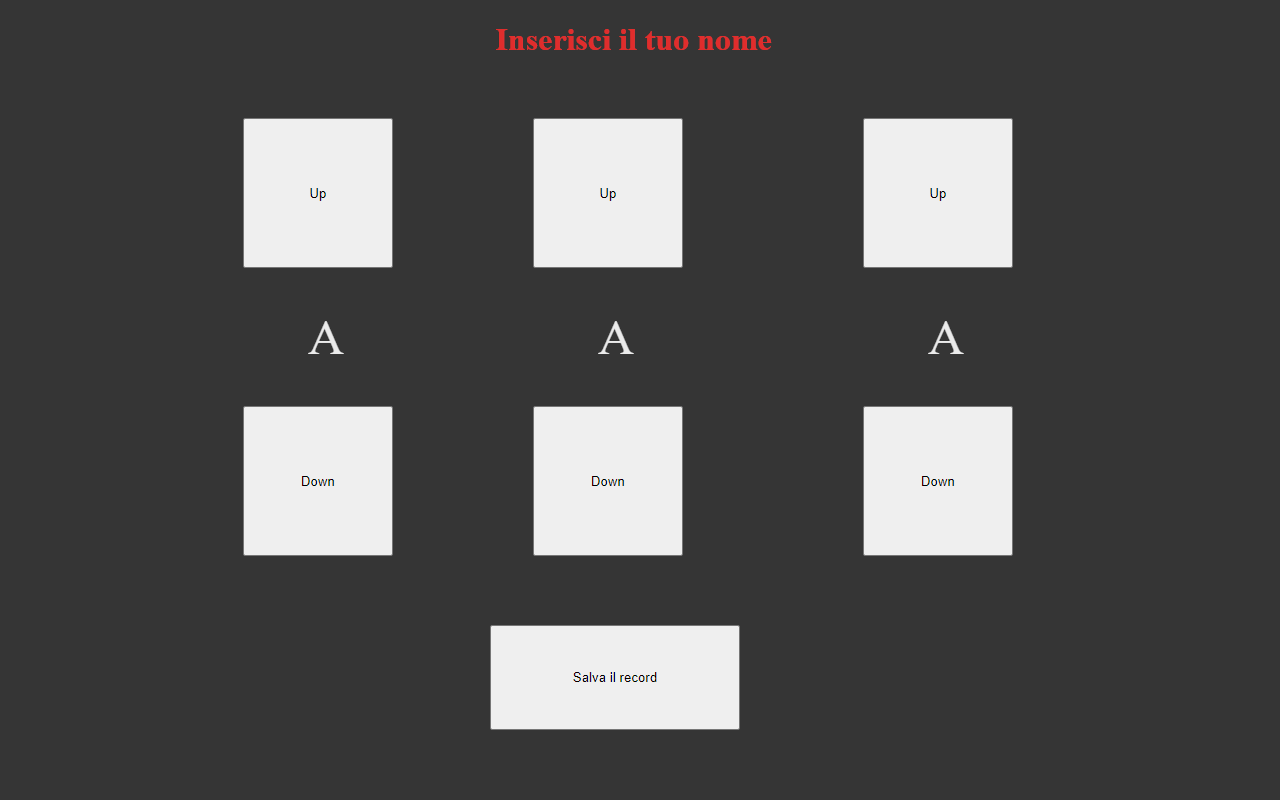
\includegraphics[width=250pt]{images/product/schermataInserimentoNome.png}
    \caption{Schermata per l'inserimento del nome}
    \label{fig:schermataInserimentoNome}
\end{figure}
\subsubsubsection{Inattività nell'inserimento di un nuovo nome}
Per quanto accade durante un'eventuale inattività, si rimanda alla sezione di \hyperref[sec:inactivity]{Gestione dell'inattività}
\newpage
\subsection{Gestione dell'inattività}
\label{sec:inactivity}
L'applicazione, se non rileva alcun input per 10 secondi, fa partire un timer di inattività della durata massima di 4 minuti. Tale timer si azzera se durante questo lasso di tempo riceve un input.\\
Nel caso scada il tempo, il sistema chiude l'attività in esecuzione (gioco o salvataggio del record) e ritorna alla schermata principale.\\
Tale azione comporta la perdita di un eventuale record effettuato, in quanto l'attività precedentemente in esecuzione viene chiusa forzatamente.